\section{Engineering Background}
% REVISIT: Write more stuff for engineering background
% research on possible architectures
% hardware of FPGA
% speed of memory
% launch registers
% PLLs
% HLS vs Verilog?
% LFSR

\subsection{Testbench Architecture}

% REVISIT: find more testbench architectures
While there has been many similar performance analysis done on hybrid SoCs
before, each of them uses their own, usually ad hoc, testbench
design~\cite{Shi1}.
This project will use a generic structure that is inspired by the structure of
an agent in UVM~\cite{Accellera1}.

\begin{figure}[H]
  \centering
  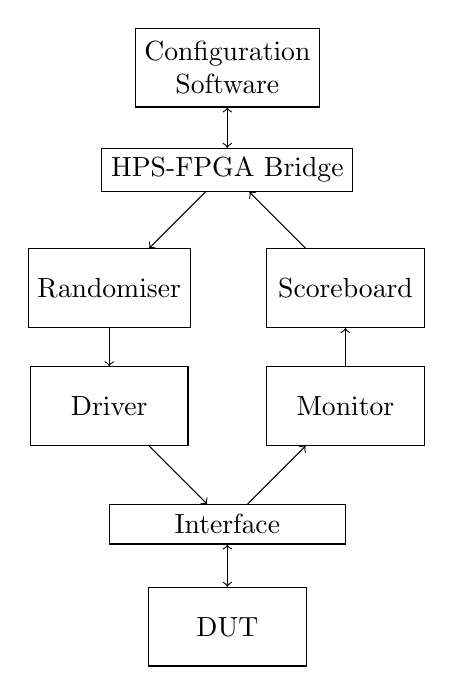
\begin{tikzpicture}
    \tikzset{block/.style= {draw,
                            rectangle,
                            align=center,
                            minimum width=2cm,
                            minimum height=1cm},
             inter/.style= {draw,
                            rectangle,
                            minimum width=3cm,
                            minimum height=0.5cm},
            }
    \path
    (0,3.5)    node[block](r) {Randomiser}
    (0,2)      node[block](d) {Driver}
    (1.5,0.5)  node[inter](i) {Interface}
    (1.5,-0.8) node[block](t) {DUT}
    (3,3.5)    node[block](s) {Scoreboard}
    (3,2)      node[block](m) {Monitor}
    (1.5,5)    node[inter](b) {HPS-FPGA Bridge}
    (1.5,6.3)  node[block](w) {Configuration\\Software}
    ;
    \draw[->]  (r) -- (d);
    \draw[->]  (d) -- (i);
    \draw[<->] (i) -- (t);
    \draw[->]  (i) -- (m);
    \draw[->]  (m) -- (s);
    \draw[->]  (b) -- (r);
    \draw[->]  (s) -- (b);
    \draw[<->] (b) -- (w);
\end{tikzpicture}
  \caption{Proposed testbench block diagram}
  \label{Block}
\end{figure}

\subsection{Target}
The design of the verification system is the major engineering challenge of this
project.
In order to stress the DUT, the verification system must perform at a much
higher frequency than the expected frequency of the DUT.
Assuming the DUT is to run at 300MHz, to fully explore the effect of
overclocking, the testbench must be able to run at double the frequency or
higher.
This gives a target frequency of 800MHz.
Assuming data width of 32-bits, the target data transfer rate is then 
This required data transfer rate is estimated to be 25.6Gbps.

\subsection{Data Transfer Rate}
% REVISIT: possible to find exact bandwidth of the bridge?
As the test is to be run on the HPS, the HPS-FPGA bridge will be the
immediate bottleneck if the test data is to flow from HPS to FPGA.
While HPS is able to easily generate test data,
there is a large amount of overhead as data crosses from one architecture
to another.
This overhead exists in terms of both a lowered bandwidth and a high delay.
Thus, it would not be sensible for HPS to send out data during run-time.

% --- using SDRAM
Another thought may be to first populate the off-chip DDR SDRAM on FPGA
side, then feed the data from there to the DUT during test.
This is already much faster than passing the data from HPS.
The 1GB, 32-bits wide DDR3 on FPGA side is rated at 400MHz.
With double rate transfer, this would gives a maximum transfer rate of 25.6Gbps.

While using the off-chip RAM may theoretically achieve the targets,
it still has its disadvantages.
First, the process of filling up the memory and then using them for the tests
takes time.
This means the test would be broken up into bursts with time in between for
checking the results and filling up with new data.
The complexity of the SDRAM interface also requires a SDRAM controller to be
used to manage SDRAM refresh cycles, address multiplexing and interface timing.
These all adds up to a significant access latency.
While this could be overcame with burst accesses and piplined accesses,
it would further complicate the SDRAM controller.
While this controller is provided by Altera~\cite{Altera3}, it is consumes
a non-negligible amount of the limited FPGA resources, while adding
unnecessary complexity to the design.
Customising the controller to fit this project may also be time-consuming.

% --- on-chip memory
The on-chip memory is much faster and simpler to handle.
This memory is implemented on the FPGA itself, and thus there is no external
connections for access to this memory.
It has the highest possible throughput, with the lowest possible latency
in an FPGA-based system.
The memory transactions can also be piplined, giving one transaction per
clock cycle.
With an on-chip FIFO accessed in dual-port mode, the write at one end and the
reads at the other end can happen simultaneously.
This effective doubling of the bandwidth is useful as tests are prepared
and fed into the DUT, or when test results are collected and fed to a checker.

On-chip memory is not without its drawbacks.
It is volatile and very limited in capacity.
While the off-chip can have its storage reaching 1GB, that of the on-chip
memory could only reach a few MB~\cite{Altera2}.
Volatility is not exactly of concern in this project, but its small capacity
means not much test data can be held before it needs more fed in.

% Looking at the options listed above, with a way of generating test data at
% run-time on the FPGA, using on-chip memory would be the most sensible option.
% REVISIT: Explain how test data could be generated at run-time

\subsection{Run-time Test Data Generation}
To exploit the benefits of using on-chip memory, a way of generating test data
at run-time needs to be designed.
As arithmetic operators have a vast set of valid inputs, it is necessary to
have cost effective test generation.

A good choice here is the use of random testing.
With relatively minimum effort, random testing can provide significant coverage
and discover relatively subtle errors~\cite{Duran1}.
% random test should be accompanied by specific tests
The main drawback of random testing is the possible lack of coverage on extreme
cases, and the usual solution is to provide handwritten tests to complement
random testing.
However, as the main goal of this testbench is mainly gauging the performance of
the module and not necessarily verifying the correctness of the arithmetic
module, this could be ignored during stress testing.
If logic correctness testing is later required, these special tests could be
written and run separately at a slower speed.

LFSRs are a reliable way of generating pseudo random numbers fast with minimum
cost~\cite{Hazwani1}.
They will thus form the starting point of data generation.
While this should not be the case for most benchmarks in this project, if some
of the data is invalid, they can be dealt with at the monitor.

With this, the software would only need to configure the randomiser, and is
no longer required to produce testing data itself.

\subsection{Clock Domains}
Another concern in the system design is of the different clock domains that
must exist on the FPGA.
At a minimum, there needs to be two clock domains, one surrounds the DUT and
another supports the rest of the control logic around the DUT.
These clock frequencies can be generated and distributed with PLLs provided as
an IP in the Quartus software~\cite{Altera4}.
Data crossing clock domains will be fed across FIFOs to prevent loss.

The proposed structure will have the driver and monitor modules running under
the same clock domain as the DUT, but the randomiser and the scoreboard does
not have to.
This means the rest of the system can be running at a slower frequency without
bottlenecking the system, thus allowing the DUT to be stressed further.

To run at a high frequency, the driver and the monitor are both simple modules.
The driver converts the stream of random numbers into inputs for the DUT, and
the monitor takes the output to check if they are correct.
% REVISIT: explain how the monitor would keep up with the high frequency

\subsection{Results Analysis}
If the monitor detects an interesting event such as an error, it will sent out
a message to the scoreboard.
The scoreboard has counters tracking these events, and update them back to the
software periodically.

The software can run statistics to provide further insights to the user.